%%% Hlavní soubor. Zde se definují základní parametry a odkazuje se na ostatní části. %%%

%% Verze pro jednostranný tisk:
% Okraje: levý 40mm, pravý 25mm, horní a dolní 25mm
% (ale pozor, LaTeX si sám přidává 1in)
\documentclass[12pt,a4paper]{report}
\setlength\textwidth{145mm}
\setlength\textheight{247mm}
\setlength\oddsidemargin{15mm}
\setlength\evensidemargin{15mm}
\setlength\topmargin{0mm}
\setlength\headsep{0mm}
\setlength\headheight{0mm}
% \openright zařídí, aby následující text začínal na pravé straně knihy
\let\openright=\clearpage

%% Pokud tiskneme oboustranně:
% \documentclass[12pt,a4paper,twoside,openright]{report}
% \setlength\textwidth{145mm}
% \setlength\textheight{247mm}
% \setlength\oddsidemargin{15mm}
% \setlength\evensidemargin{0mm}
% \setlength\topmargin{0mm}
% \setlength\headsep{0mm}
% \setlength\headheight{0mm}
% \let\openright=\cleardoublepage

%% Použité kódování znaků: obvykle latin2, cp1250 nebo utf8:
\usepackage[utf8]{inputenc}

%% Ostatní balíčky
\usepackage{graphicx}
\usepackage{amsthm}

%% My packages:
\usepackage{algorithm}
\usepackage{algpseudocode}
\usepackage{commath}
\usepackage{float}
\floatstyle{ruled} \newfloat{pseudocode}{thp}{lop} \floatname{pseudocode}{Pseudocode}
\usepackage{color}
\definecolor{lightgray}{rgb}{0.95, 0.95, 0.95}
\definecolor{darkgray}{rgb}{0.4, 0.4, 0.4}
\definecolor{purple}{rgb}{0.65, 0.12, 0.82}
\definecolor{editorGray}{rgb}{0.95, 0.95, 0.95}
\definecolor{editorOcher}{rgb}{1, 0.5, 0} % #FF7F00 -> rgb(239, 169, 0)
\definecolor{editorGreen}{rgb}{0, 0.5, 0} % #007C00 -> rgb(0, 124, 0)
\usepackage{upquote}
\usepackage{listings}
% CSS
\lstdefinelanguage{CSS}{
  keywords={color,background-image:,margin,padding,font,weight,display,position,top,left,right,bottom,list,style,border,size,white,space,min,width, transition:, transform:, transition-property, transition-duration, transition-timing-function},	
  sensitive=true,
  morecomment=[l]{//},
  morecomment=[s]{/*}{*/},
  morestring=[b]',
  morestring=[b]",
  alsoletter={:},
  alsodigit={-}
}

% JavaScript
\lstdefinelanguage{JavaScript}{
  morekeywords={typeof, new, true, false, catch, function, return, null, catch, switch, var, if, in, while, do, else, case, break},
  morecomment=[s]{/*}{*/},
  morecomment=[l]//,
  morestring=[b]",
  morestring=[b]'
}

\lstdefinelanguage{HTML5}{
  language=html,
  sensitive=true,	
  alsoletter={<>=-},	
  morecomment=[s]{<!-}{-->},
  tag=[s],
  otherkeywords={
  % General
  >,
  % Standard tags
	<!DOCTYPE,
  </html, <html, <head, <title, </title, <style, </style, <link, </head, <meta, />,
	% body
	</body, <body,
	% Divs
	</div, <div, </div>, 
	% Paragraphs
	</p, <p, </p>,
	% scripts
	</script, <script,
  % More tags...
  <canvas, /canvas>, <svg, <rect, <animateTransform, </rect>, </svg>, <video, <source, <iframe, </iframe>, </video>, <image, </image>
  },
  ndkeywords={
  % General
  =,
  % HTML attributes
  charset=, src=, id=, width=, height=, style=, type=, rel=, href=,
  % SVG attributes
  fill=, attributeName=, begin=, dur=, from=, to=, poster=, controls=, x=, y=, repeatCount=, xlink:href=,
  % CSS properties
  margin:, padding:, background-image:, border:, top:, left:, position:, width:, height:,
	% CSS3 properties
  transform:, -moz-transform:, -webkit-transform:,
  animation:, -webkit-animation:,
  transition:,  transition-duration:, transition-property:, transition-timing-function:,
  }
}

\lstset{%
  % General design
  backgroundcolor=\color{editorGray},
  basicstyle={\small\ttfamily},   
  frame=l,
  % line-numbers
  xleftmargin={0.75cm},
  numbers=left,
  stepnumber=1,
  firstnumber=1,
  numberfirstline=true,	
  % Code design
  identifierstyle=\color{black},
  keywordstyle=\color{blue}\bfseries,
  ndkeywordstyle=\color{editorGreen}\bfseries,
  stringstyle=\color{editorOcher}\ttfamily,
  commentstyle=\color{darkgray}\ttfamily,
  % Code
  language=HTML5,
  alsolanguage=JavaScript,
  alsodigit={.:;},	
  tabsize=2,
  showtabs=false,
  showspaces=false,
  showstringspaces=false,
  extendedchars=true,
  breaklines=true,
  % German umlauts
  literate=%
  {Ö}{{\"O}}1
  {Ä}{{\"A}}1
  {Ü}{{\"U}}1
  {ß}{{\ss}}1
  {ü}{{\"u}}1
  {ä}{{\"a}}1
  {ö}{{\"o}}1
}
\usepackage{caption}
\captionsetup[lstlisting]{position=bottom}

%%% Drobné úpravy stylu

% Tato makra přesvědčují mírně ošklivým trikem LaTeX, aby hlavičky kapitol
% sázel příčetněji a nevynechával nad nimi spoustu místa. Směle ignorujte.
\makeatletter
\def\@makechapterhead#1{
  {\parindent \z@ \raggedright \normalfont
   \Huge\bfseries \thechapter. #1
   \par\nobreak
   \vskip 20\p@
}}
\def\@makeschapterhead#1{
  {\parindent \z@ \raggedright \normalfont
   \Huge\bfseries #1
   \par\nobreak
   \vskip 20\p@
}}
\makeatother

% Toto makro definuje kapitolu, která není očíslovaná, ale je uvedena v obsahu.
\def\chapwithtoc#1{
\chapter*{#1}
\addcontentsline{toc}{chapter}{#1}
}

%\usepackage{color}
\definecolor{lightgray}{rgb}{0.95, 0.95, 0.95}
\definecolor{darkgray}{rgb}{0.4, 0.4, 0.4}
\definecolor{purple}{rgb}{0.65, 0.12, 0.82}
\definecolor{editorGray}{rgb}{0.95, 0.95, 0.95}
\definecolor{editorOcher}{rgb}{1, 0.5, 0} % #FF7F00 -> rgb(239, 169, 0)
\definecolor{editorGreen}{rgb}{0, 0.5, 0} % #007C00 -> rgb(0, 124, 0)
\usepackage{upquote}
\usepackage{listings}
% CSS
\lstdefinelanguage{CSS}{
  keywords={color,background-image:,margin,padding,font,weight,display,position,top,left,right,bottom,list,style,border,size,white,space,min,width, transition:, transform:, transition-property, transition-duration, transition-timing-function},	
  sensitive=true,
  morecomment=[l]{//},
  morecomment=[s]{/*}{*/},
  morestring=[b]',
  morestring=[b]",
  alsoletter={:},
  alsodigit={-}
}

% JavaScript
\lstdefinelanguage{JavaScript}{
  morekeywords={typeof, new, true, false, catch, function, return, null, catch, switch, var, if, in, while, do, else, case, break},
  morecomment=[s]{/*}{*/},
  morecomment=[l]//,
  morestring=[b]",
  morestring=[b]'
}

\lstdefinelanguage{HTML5}{
  language=html,
  sensitive=true,	
  alsoletter={<>=-},	
  morecomment=[s]{<!-}{-->},
  tag=[s],
  otherkeywords={
  % General
  >,
  % Standard tags
	<!DOCTYPE,
  </html, <html, <head, <title, </title, <style, </style, <link, </head, <meta, />,
	% body
	</body, <body,
	% Divs
	</div, <div, </div>, 
	% Paragraphs
	</p, <p, </p>,
	% scripts
	</script, <script,
  % More tags...
  <canvas, /canvas>, <svg, <rect, <animateTransform, </rect>, </svg>, <video, <source, <iframe, </iframe>, </video>, <image, </image>
  },
  ndkeywords={
  % General
  =,
  % HTML attributes
  charset=, src=, id=, width=, height=, style=, type=, rel=, href=,
  % SVG attributes
  fill=, attributeName=, begin=, dur=, from=, to=, poster=, controls=, x=, y=, repeatCount=, xlink:href=,
  % CSS properties
  margin:, padding:, background-image:, border:, top:, left:, position:, width:, height:,
	% CSS3 properties
  transform:, -moz-transform:, -webkit-transform:,
  animation:, -webkit-animation:,
  transition:,  transition-duration:, transition-property:, transition-timing-function:,
  }
}

\lstset{%
  % General design
  backgroundcolor=\color{editorGray},
  basicstyle={\small\ttfamily},   
  frame=l,
  % line-numbers
  xleftmargin={0.75cm},
  numbers=left,
  stepnumber=1,
  firstnumber=1,
  numberfirstline=true,	
  % Code design
  identifierstyle=\color{black},
  keywordstyle=\color{blue}\bfseries,
  ndkeywordstyle=\color{editorGreen}\bfseries,
  stringstyle=\color{editorOcher}\ttfamily,
  commentstyle=\color{darkgray}\ttfamily,
  % Code
  language=HTML5,
  alsolanguage=JavaScript,
  alsodigit={.:;},	
  tabsize=2,
  showtabs=false,
  showspaces=false,
  showstringspaces=false,
  extendedchars=true,
  breaklines=true,
  % German umlauts
  literate=%
  {Ö}{{\"O}}1
  {Ä}{{\"A}}1
  {Ü}{{\"U}}1
  {ß}{{\ss}}1
  {ü}{{\"u}}1
  {ä}{{\"a}}1
  {ö}{{\"o}}1
}

\usepackage{footnote}
\usepackage{array}
\newcolumntype{L}[1]{>{\raggedright}m{#1}}
\newcolumntype{C}[1]{>{\centering}m{#1}}

\newcommand{\footnoteremember}[2]{
\footnote{#2}
\newcounter{#1}
\setcounter{#1}{\value{footnote}}
}
\newcommand{\footnoterecall}[1]{
\footnotemark[\value{#1}]
}


\usepackage[refpage]{nomencl}
\usepackage{etoolbox}
\makeatletter
\patchcmd{\thenomenclature}%
  {\chapter*{\nomname}}%
  {\section*{\nomname}}%
  {}{\message{^^Jthenomenclature patching failed (1)^^J}}
\patchcmd{\thenomenclature}%
  {\if@intoc\addcontentsline{toc}{chapter}{\nomname}\fi}%
  {\if@intoc\addcontentsline{toc}{section}{\nomname}\fi}%
  {}{\message{^^Jthenomenclature patching failed (2)^^J}}
\makeatother
\makenomenclature
\renewcommand{\nomname}{} % empty name

\usepackage{pdfpages}



%% Balíček hyperref, kterým jdou vyrábět klikací odkazy v PDF,
%% ale hlavně ho používáme k uložení metadat do PDF (včetně obsahu).
%% POZOR, nezapomeňte vyplnit jméno práce a autora.
\usepackage[ps2pdf,unicode]{hyperref}   % Musí být za všemi ostatními balíčky
%\usepackage[unicode]{hyperref}   % Musí být za všemi ostatními balíčky
\hypersetup{pdftitle=Vector Screencast}
\hypersetup{pdfauthor=Šimon Rozsíval}


\begin{document}

% Trochu volnější nastavení dělení slov, než je default.
\lefthyphenmin=2
\righthyphenmin=2

%%% Titulní strana práce

\pagestyle{empty}
\begin{center}

\large

Charles University in Prague

\medskip

Faculty of Mathematics and Physics

\vfill

{\bf\Large BACHELOR THESIS}

\vfill

\centerline{\mbox{\includegraphics[width=60mm]{../img/logo.eps}}}

\vfill
\vspace{5mm}

{\LARGE Šimon Rozsíval}

\vspace{15mm}

% Název práce přesně podle zadání
{\LARGE\bfseries Vector Screencast}

\vfill

% Název katedry nebo ústavu, kde byla práce oficiálně zadána
% (dle Organizační struktury MFF UK)
Department of Distributed and Dependable Systems

\vfill

\begin{tabular}{rl}

Supervisor of the bachelor thesis: & Mgr. Martin Děcký \\
\noalign{\vspace{2mm}}
Study programme: & Computer science \\
\noalign{\vspace{2mm}}
Specialization: & Programming and software systems \\
\end{tabular}

\vfill

% Zde doplňte rok
Prague 2015

\end{center}

\newpage

%%% Následuje vevázaný list -- kopie podepsaného "Zadání bakalářské práce".
%%% Toto zadání NENÍ součástí elektronické verze práce, nescanovat.

%%% Na tomto místě mohou být napsána případná poděkování (vedoucímu práce,
%%% konzultantovi, tomu, kdo zapůjčil software, literaturu apod.)

\openright

\noindent
I would like to thank my supervisor, Martin Děcký, for his valuable pieces of advice, and Otakar Jícha from \textit{Khanova Škola}, for the idea of this project and for lending me a graphics tablet for testing.

I would also like to thank my family and friends for supporting me during my studies.



\newpage

%%% Strana s čestným prohlášením k bakalářské práci

\vglue 0pt plus 1fill

\noindent
I declare that I carried out this bachelor thesis independently, and only with the cited
sources, literature and other professional sources.

\medskip\noindent
I understand that my work relates to the rights and obligations under the Act No.
121/2000 Coll., the Copyright Act, as amended, in particular the fact that the Charles
University in Prague has the right to conclude a license agreement on the use of this
work as a school work pursuant to Section 60 paragraph 1 of the Copyright Act.

\vspace{10mm}

\hbox{\hbox to 0.5\hsize{%
In ........ date ............
\hss}\hbox to 0.5\hsize{%
signature of the author
\hss}}

\vspace{20mm}
\newpage

%%% Povinná informační strana bakalářské práce

\vbox to 0.5\vsize{
\setlength\parindent{0mm}
\setlength\parskip{5mm}

Název práce:
Vektorový screencast
% přesně dle zadání

Autor:
Šimon Rozsíval

Katedra:  % Případně Ústav:
Katedra distribuovaných a spolehlivých systémů
% dle Organizační struktury MFF UK

Vedoucí bakalářské práce:
Mgr. Martin Děcký
% dle Organizační struktury MFF UK, případně plný název pracoviště mimo MFF UK

Abstrakt:
Cílem bakalářské práce je vytvořit software pro záznam a přehrávání výukových videí pro potřeby Khanovy školy. Na rozdíl od běžných videí nejsou obrazová data uložena ve formě bitmap, ale jako vektory, což umožní snížit datovou náročnost a vykreslit obraz ostře při libovolně velkém rozlišení obrazovky uživatele. Přehrávač videa i nástroj pro nahrávání běží ve webovém prohlížeči. Součástí práce je také návrh a implementace vhodného formátu pro uchovávání obrazových a zvukových dat a implementace v softwarové architektuře klient/server.
% abstrakt v rozsahu 80-200 slov; nejedná se však o opis zadání bakalářské práce

Klíčová slova:
screencast, vektory, video, on-line

\vss}\nobreak\vbox to 0.49\vsize{
\setlength\parindent{0mm}
\setlength\parskip{5mm}

Title:
Vector Screencast

Author:
Šimon Rozsíval

Department:
Department of Distributed and Dependable Systems
% dle Organizační struktury MFF UK v angličtině

Supervisor:
Mgr. Martin Děcký
% dle Organizační struktury MFF UK, případně plný název pracoviště
% mimo MFF UK v angličtině

Abstract:
The goal of this bachelor thesis is to create a software for recording and playback of educational videos for Khanova škola (Czech clone of Khan Academy). Contrary to common videos the visual data is not stored as a sequence of bitmaps, but as vectors. This allows to reduce the data bandwidth and playback sharp images in any target resolution. The player and also the tool for recording the videos runs in a web browser. The thesis also focuses on designing and implementing a suitable file format for storing the visual and audio data and implementing the software according to the client/server paradigm.
% abstrakt v rozsahu 80-200 slov v angličtině; nejedná se však o překlad
% zadání bakalářské práce

Keywords:
screencast, vector, video, on-line
% 3 až 5 klíčových slov v angličtině

\vss}

\newpage

%%% Strana s automaticky generovaným obsahem bakalářské práce. U matematických
%%% prací je přípustné, aby seznam tabulek a zkratek, existují-li, byl umístěn
%%% na začátku práce, místo na jejím konci.

\openright
\pagestyle{plain}
\setcounter{page}{1}
\tableofcontents

%%% Jednotlivé kapitoly práce jsou pro přehlednost uloženy v samostatných souborech
\chapter*{Introduction}
\addcontentsline{toc}{chapter}{Introduction}
A year ago two members of ``Khanova škola'', the Czech brach of the Khan Academy, came with an idea of improving the current technical solution of recording and displayling educational videos on their website. It turns out that some of the videos recorded only a few years ago don't look very well or the hand-drawn text in these videos is not even legible on large displays. The other extreme are small displays of tablets and smartphones, where the downscaled letters are too small to read and can't be zoomed well in most video players. Their idea was to create a vector-based animation instead of classical bitmap-based screencasts. This animation could be scaled to any display resolution without any loss of information. The process of recording can be simulated in any distant future based on the recorded data of user's behaviour. The animation can be rendered using a different algorithm and the author would not have to record his screen again. As a result, the video will never become obsolete because of its poor visual quality.

One of the other reasons for this type of solution was the possible decrease of the size of data transfered over the Internet, as most of the image does not change between each two frames and very often the image doesn't change at all. The file size of a vector-based format does not correspond to the quality of the video. In regular bitmap formats, the higher the resolution of an image is, the the larger the data file is. Vector-based format has only one version for every display resolution.

\section*{Khan Academy}
\label{sec:khan-academy}
The idea of \textit{Khan Academy} originated in 2003 when Salman Khan began tutoring his cousin over an instant messenger via drawing pictures with a computer mouse. Salman then started to record these videos and put them on his Youtube channel, so someone could watch them later. This channel became the basis of Khan Academy.

Khan Academy became known and has grown a lot, but the style of Khan Academy videos remained the same. A person draws lines and diagrams using a bitmap editor on his computer and talks about the subject aloud while recording his computer screen and recording his voice using a microphone. This style is sometimes called the ``Khan-style video'' (KSV)\nomenclature{KSV}{Khan-style video} \footnote{https://www.youtube.com/watch?v=Ohu-5sVux28}. These videos are then uploaded to Youtube and embedded in the Khan Academy website.

Apart from the video lectures, the website also contains exercises and quizzes to encourage students in learning. The pace of the lesson depends on the student. He can pause the videos or watch them multiple times before continuing with the lesson.

Most of the videos are recorded in English, but many of the videos are translated into other languages - by replacing the audio track with a different one or with subtitles. One of the projects working on the localization of Khan Academy videos is an official Czech branch called ``Khanova Škola''.

\subsection*{``Khanova Škola''}
\textit{Khanova Škola} is the Czech branch of the Khan Academy \cite{khanova_skola}. It is a non-profit organization. Volunteers around ``Khanova Škola'' translate the original videos from English to Czech to make them accessible for children at Czech elementary schools.

\subsection*{Screencast}
A screencast is a video created by recording computer screen output, often accompanied with an audio commentary. This process can be used in many different ways, for example to record a tutorial explaining how to use a specific computer program. The quality of the recorded video depends mainly on the resolution of the user's device resolution and the recorded area of the screen. Khan Academy uses screen capturing tools to record the virtual canvas of a bitmap editor, onto which the author draws using the tools of the editor and talks about the covered subject.

\section*{Goal of the thesis}
\addcontentsline{toc}{section}{Goal of the thesis}

The result of this thesis should be an open-source library suitable for extending any web application, like ``Khanova Škola'', with the abilities of recording and playing KSVs in all modern web browsers. Screencast will be recorded and played using a technology based on vector graphics to guarantee the quality of the video on any display and to achieve lower file size of the video file. An appropriate vector-based file format should be chosen or defined to store screencast data.

The library should be easily adjustable and configurable for different purposes. User interface should be fully translatable.

\section*{Thesis structure}
\addcontentsline{toc}{section}{Thesis structure}
The first part of the thesis is about distance education in general. Reader should get a notion of current distance education systems and their limits.

The technical requirements of the project are described in the following chapter. The third chapter is the analysis of the available tools and algorithms and which approaches to choose. A file format for the puroposes of this project is defined and described afterwards.

Following chapters contain information about the implementation of the library and its components, how the library can be integrated into websites, and how to use the library to record and play screencasts.
\chapter{Distance education}

Distance education is not only a phenomenon of the few last decades, but can be traced at least back to the 18th century, when Caleb Phillipps posted an advertisment called ``Teacher of the New Method of Short Hand'' in Boston Gazette, saying ``Persons in the Country desirous to Learn this Art, may by having the several Lessons sent weekly to them, be as perfectly instructed as those that live in Boston.'' \cite{1}

With the development of the Internet and its general accessibility in the developed world, providing distance education has become much easier and has spread widely. In some countries tuition rates are high and young people take loans. This topic is covered in a fitting way by John Oliver in his show \cite{2}. The flexibility and low cost of distatnce education over the Internet gives people, who wouldn't be otherwise able to attend a traditional university, an opportunity to gain knowledge and train skills from their homes \cite{3}.

Students in the deveopling world are also taking the advantage of educational content available on the Internet. Several of the top U.S. universities, like Harvard, Stanford or MIT, put some of their materials on so called MOOCs (Massive Open Online Course) like Coursea, edX or Udacity. This content is then available to anyone with a computer and Internet connection and knowledge of the language. A fitting example is Kepler - non profit university project in Rwanda \cite{5}. The goal of this project is to ``provide an American-accredited degree, a world class education, and a clear path to good jobs for thousands of students for around \$1,000 tuition per year.'' \cite{6}

\section{Current systems}
In the next few pragraph I will try to pick some of the current distance education systems available on the Internet for free. This list is not complete and is only meant to give the reader a notion of available technologies and their paradigms, which project into the project of Vector Screencast.

\subsection{Moodle}
Moodle \cite{7} is an open-source project providing a robust tool for creating custom learning materials and providing them to students. Anyone can download the source code of Moodle and deploy it on his own server.

This tool is used by millions of users \cite{8}.

\subsection{Coursera}
The mission of Coursera is to ``provide universal access to the world’s best education.'' \cite{9} Anyone can, for free, go through materials published by universities and other organizations aimed at education.

Courses at Coursera consist mainly of video lectures commonly with a transcript and a presentation document attached to. These videos can be viewed directly in the browser on demand or downloaded to user's computer. After studing the materials, students can submit asignments solutions and take quizes and receive a Verified Certificate for the accomplishement of the course. These certificates are not free.

Most of the courses are in English and only a few of the courses are also translated into other languages. It is not possible for everyone to publish his materials through Coursera.

\subsection{Youtube.com}
The Youtube web service \cite{10} is not primarily designed to be an educational resource. Youtube allows people to create their own video content and share it with other Internet users for free. Youtube was launched in 2005 and has became one of the most frequently visited websites on the Internet according to Alexa Internet \cite{11}. Uploading video to Youtube is free, advertisment is displayed to the user while watching videos though.

The ease of making original-created videos available and the wide audience makes Youtube a perfect place for all individuals and organizations, who want to share their ideas or any video materials. Many educational channels can be found here, for example Numberphile \cite{12}, Veritasium \cite{13}, and Khan Academy \cite{14}.

Youtube videos can be viewed only online in a web browser or a specialized application. There are only unofficial tools for downloading these videos.

The form and content of the video is not limited anyhow, as long as does not violate the terms of the service. Video can have a text description which might contain the transcription of the video content and any subtitles can be attached to a video. Youtube also downscales videos to multiple resolutions so they can be also viewed using low speed Internet connections.

\subsection{Khan Academy}
A similar service to Coursera is Khan Academy. Khan Academy originated in 2004 when it's founder, Salman Khan, began tutoring his cousin over an instant messenger via drawing diagrams with a computer mouse. Salman then started to capture these videos and put them on Youtube, so someone could watch them later.

The format of Khan Academy videos remained the same. A person draws diagrams on a computer canvas and comments the subject with his voice. These videos are then uploaded to Youtube and embeded on the Khan Academy website \cite{14}. Apart form the video lectures, the website also contains exercises and quizes to encourage students in learning. The pace of the lesson depends on the student. He can pause the videos or watch them multiple times before continuing with the lesson~\ref{fig:khan-screen}.

Most of the videos are recorded in English, but many of the videos are translated into other languages - by replacing the audio track with a different one or with subtitles.

One of the projects working on the localization of Khan Academy videos is a czech branch called Khanova Škola \cite{15}.

\begin{figure}
	\centering
	%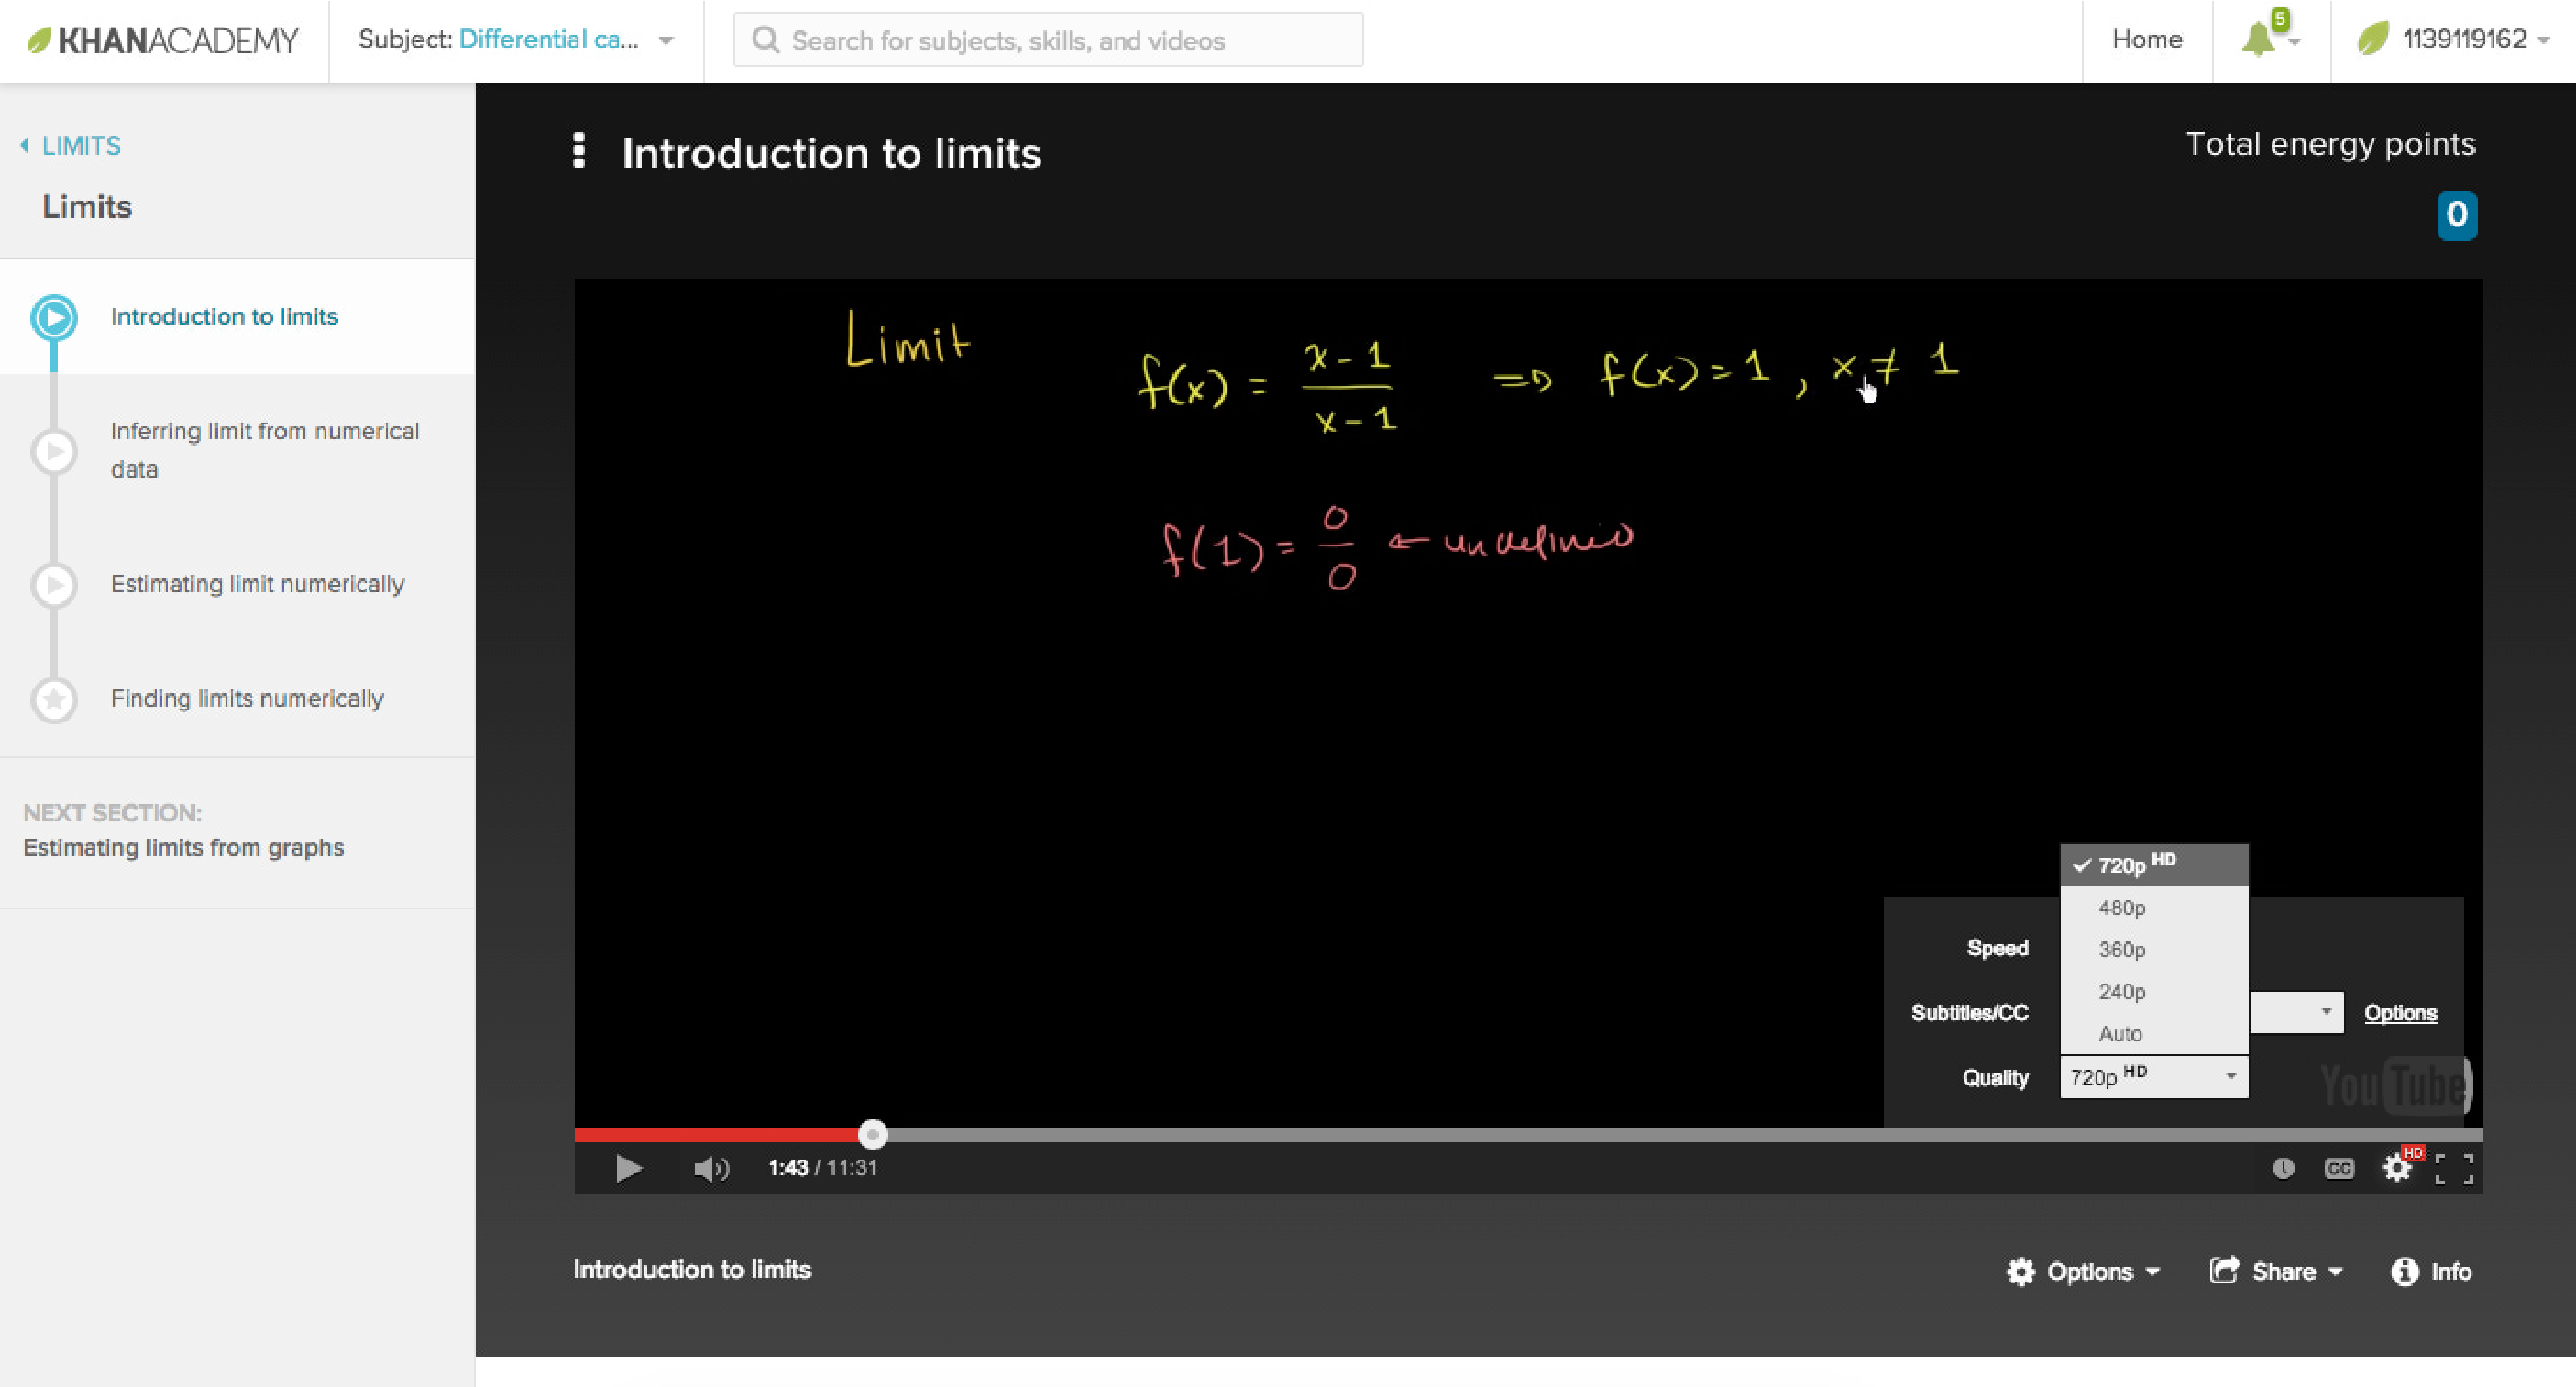
\includegraphics[width=30mm]{../img/khan-academy-screenshot.png}
	\caption{Khan Academy lesson}
	\label{fig:khan-screen}
\end{figure}
\chapter{The Vector Video project}

In the spring of 2014 the people behind ``Khanova Škola'' -- the Czech branch of the Khan Academy -- were looking for a person to develop an experimental video technology based on vector graphics. Their idea was to record raw data of user's input as he creates a Khan-style-video and later, when another user watches the video, draw the video scaled to match user's device's resolution and thus achieving maximum quality of the output. The result of this will be that the video will never become obsolete because it's quality isn not keeping up with the times.

Thanks to the sparse nature of vectors, in comparison to bitmaps, the data consumption might also be reduced or at least similar. This animation would also be linked to an audio track of authors voice commentary forming a complex KSV video suitable for educational purposes.

\section{Video recording tool requirements}
User, who wants to create a new video, should enter a website in his web browser and without installing any additional software start recording a video using his mouse, touchscreen or digital stylus and a microphone. This video should then be uploaded to the server.

If the user uses a pressure-sensitive stylus, then the applied pressure during drawing should be recorded too. The more pressure the user applies, the thicker the line will be and vice versa. Using this specific hardware might require additional drivers or specific software installed.

Different brush sizes, brush colors and background colors are available for the user. User should be able to erase certain parts of the canvas or the whole canvas at once. User should be able to pause and continue recording at any time.

Lines are immediately rendered on the screen as the user draws them, so he sees exactly the same output as the viewer will when he is playing the video later. All the raw data collected from the user should be stored, including the data that have no effect for video playback, like recording cursor movement while recording is paused. This will allow the user to simulate the process of video recording in the future and use it for further post-processing in any distant future. Recording of this redundant information should be optional.

\section{Video player requirements}
Any user should be able to play vector video on-line in all major modern web browsers without any special software or plugin installed, including mobile browsers.

Video should be scaled appropriately to the size of the player and device's screen resolution. The lines should have the same shape as the author has intended.

User can pause and continue with the playback of the video at any time. User can skip to any point of the video either forward or backward.

If the author of the video had recorded his voice, it must be played along the video. Audio must be synchronized with the video whenever user plays or pauses the video or when he skips to a different point on the time line.

User interface should be intuitive and easy to use either on a desktop computer using mouse and keyboard, but also with touchscreens on mobile devices.

\section{Goal of this thesis}

The result of this thesis should be an open-source library suitable for extending any web application with the abilities of recording and playing Khan Academy style videos in modern web browsers. An appropriate vector-based format should be chosen or defined to store video data.

The library should be easily adjustable and configurable for different purposes. User interface should be fully translatable to any language.
\chapter{Analysis}

\subsection{Technical requirements}
The overall project consists of two separate tools --- the recorder and the player. Each of these tools behaves differently and will be used by different people. While the video player will be used by general audience, the recorder will be used by a much narrower group of content creators.

The recording tool will capture the movement of a virtual chalk and lines drawn on a virtual blackboard, as well as voice of the author using a microphone. The recorder data will be then sent to the server, where it should be stored. The video player will receive previousely recorded data and display the movement of the chalk and lines created by the author while playing the voice comment. It is required that the video player will placed in a web page and it must run well in a all modern web browsers without requiring installation of any non-standard plugins or codecs and thus making it easy for a potential viewer to watch contents of the video.

For the purposes of recording, the tool must be able to capture the input from a microphone, track mouse movement and left mouse button state, collect information from Wacom graphics tablet devices and draw lines on screen. What the creator sees should be the same as what the end user will watch later.

\subsection{Available techonologies}
Web is a huge and fast growing environment. In only a few years, it has become a universal place for exchanging and presenting information. This put the web in the focus of many software companies and organizations and as a result, many different technologies for developing rich interactive applications (RIA) have been created. Some of them have already faded into obscurity, other are just emerging. One of the main limitations in the selection of the right technology for developing web application is their compatibility with operating systems and web browsers.

\subsubsection{Java applets}
Java applets are used for creating interactive applications withing web browser. Java applets meet all the specified technical requirements of both video player and recording tool.

Java applets are written in any language, that can be compiled into bytecode, this bytecode is then downloaded to the web browser and then run using Java Virtual Machine (JVM). This means that to be able to run a Java applet, user needs to have JVM installed on the device and an installed and allowed Java plugin in user's browser. This isn't a problem for desktop systems as Java is open source, but there is no support for mobile operating systems such as iOS and Android \cite{}. 

\subsubsection{Adobe Flash}
Adobe Flash is a multimedia and software platform used for creating vector graphics, animations and games. Flash has all required features: vector graphics manipulation, working with XML, mouse input capturing, microphone input, and audio streaming \cite{}. 

To view Flash animations or to execute Flash applications, Adobe Flash Player is needed. Adobe Flash Player is available and being developed for all major operating systems, although that is not true for mobile platforms. There was never any support for Apple iOS \cite{} and in 2012 deveolpment of Flash for Android was discontinued \cite{}. Using Adobe Flash would mean to exclude most users of tablets and smartphones \cite{}, which is a large disadvantage of this technology.

\subsubsection{Microsoft Silverlight}
Microsoft Silverlight \cite{} a development tool for creating web applications. It is based on the .NET Framework and it is similar to Java applets and Adobe Flash. It was Microsoft's attempt to compete Adobe Flash, but wasn't well adopted.

Silverlight comes as a plugin for web browsers. It is free, altough the list of supported browsers is even smaller \cite{} than the one of Adobe Flash consisting of exclusively desktop operating systems. Development of Silverlight was also discontinued by Microsoft in 2012 and the combination of these facts makes it unsuitable for this project.

\subsubsection{HTML5}
HTML5 is the fifth revision of Hypertext Markup Language (HTML) standard of World Wide Web Consortium (W3C). It has been given the Recommendation status in the end of 2014 and a significant part of it's new features is already implemented in modern web browsers.

Can I perform all needed tasks using this technology?
Player:
Audio - http://caniuse.com/#search=audio%20element
SVG - http://caniuse.com/#search=svg

Recorder: 
getUserMedia/Stream API - http://caniuse.com/#search=getUserMedia
Web Sockets - http://caniuse.com/#search=web%20sockets

\subsection{Conclusion}
The bottleneck of most of the technologies is their support in mobile devices. These devices don't allow some of the above mentioned technologies to run inside them. As the popularity and market share of mobile devices grows, supporting them is a priority. This eventually leads to only one option, and that is HTML5. All major web browsers have the features needed to create the video player, including the versions of browsers for mobile devices.

The specification of HTML5 is finished since  and support of all it's features isn't implemented in all today's web browsers. This situation is getting better with every release of a new version of all web browsers.




\subsection{Possible issues and known limitations}
About browser speed. Memory limitations. Network speed.

Mobile OS browsers limitations - audio recording.

Audio recording - large ammount of data - uncompressed - which approach of upload to choose? The most simple - create wav in browser and upload it via multipart form. The more complicated approach - continuous stream using WebSockets or WebRTC - need of specific web server process implementation.

\chapter{Vector Screencast file format}

Vector video file must contain all the information about cursor movement and precise data of the lines, including their variable width, and the times at which every single segment of a line is drawn. This data is then used to reconstruct the precise movement of the author's cursor and draw the very sqme lines at the very same pace.

There are several vector based formats available.

\paragraph{Scalable Vector Graphics (SVG)}
Scalable Vector Graphics (SVG)\footnote{http://www.w3.org/TR/SVG/} is an Extensible Markup Language (XML)\footnote{http://www.w3.org/XML/} based file format designed for describing two-dimensional vector images. It is an open format developed and maintained by the W3C SVG Working Group \cite{}. Current W3C Recommendation is SVG 1.1 (Second Edition).

A valid SVG document must have an \textit{svg} root element with specific namespace attributes and specified \textit{width} and \textit{height} attributes. An example of an empty, but valid, SVG document might look as shown:

\begin{verbatim}
<?xml version="1.0"?>
<svg version="1.1"
        width="470"
        height="100"
        xmlns="http://www.w3.org/2000/svg"
        xmlns:xlink="http://www.w3.org/1999/xlink"
        xmlns:ev="http://www.w3.org/2001/xml-events">

</svg>
\end{verbatim}

The specification of SVG introduces several graphical primitives, that can be used to compose complex shapes. Each primitive is represented by an XML element and a set of attributes. The list of primitives is long, though we will need only two of them -- the \verb|<circle>|, \verb|<rect>| and \verb|<path>|. The \verb|<g>| element\footnote{http://www.w3.org/TR/SVG/struct.html\#GElement} is intended for grouping related graphics elements. These groups might be also nested.
\chapter{Implementation}
How the source was designed and maintained. Mention that the development of the code can be found on Github?

\section{HTML5}
What is HTML5, what parts are needed. Compatibility of these technologies in browsers. A chart of people using a compatible browser? Playing should be possible in the vast majority of browsers today and the prognose is good.

\subsection{Event driven programming}
Why it is used. What are the pros and cons. How is it used in websites. How the inner implementation in Vector Screencast works.
% en.wikipedia.org/wiki/Event-driven_programming

\subsection{Working with XML data}
Using jQuery here.

\subsection{Drawing lines}
At the time of recording, mouse coordinates relative to the drawing board are captured along with the pressure of the pen on a drawing board or the state of the left mouse button. This data is then used to draw a line with a changing width at the moment of recording as a visual feedback for the person recording and then every time the video will be replayed. The outcome of the rendering phase should be the same every time so the intention of the creator is perserved. On the other hand, the rendering algorithm might be improved in the future and the video could be rendered using to this algorithm without any editing.

Rendering at the time of playback gives us the opportunity to adjust the outcome to the environment of the end user. This means that the result can be sharp on every display resolution.



\subsection{Input handling}
Detecting mouse and keyboard input is easy, there is a plugin for Wacom darwing tablets and it is supported in Vector Screencast - different pressure means different thickness.
\chapter{Using Vector Screencast library}
\label{ch:integration}

Using Vector Screencast library is intended to be as simple as possible. All the user needs to do is include a JavaScript file of the library and a CSS file of a theme into his HTML code and configure the player in a few lines of code.

\section{Obtaining the Vector Screencast library}
Prepared library files can be obtained either from the attached files or from Git repository https://github.com/simonrozsival/vectorvideo in the \verb|/release/VectorScreencast| and \verb|/release/themes/| folders. You only need to copy files \verb|vector-screencast.min.js| and \verb|theme-default.min.css| into your project.

The library files must be linked to your document and you should make sure that your website will be displayed properly on mobile devices by specifying the \verb|viewport| meta tag in the \verb|head| section of your document \cite{html_viewport}. Also create an empty element with a specific \verb|id| attribute -- this will be the container, into which either the screencast player or the recorder will be placed.

An example of a HTML5 template with correct setup can look similarly (irrelevant parts of the document were let omitted and replaced by suspension points):

\begin{lstlisting}
<!DOCTYPE html>
<html>
	<head>
		...
		<meta name="viewport" content="width=device-width,initial-scale=1">
		<link rel="stylesheet" type="text/css" href="/path/to/theme-default.min.css" media="screen, projection">
		...
	</head>
	<body>
		...
		<div id="some-specific-id"></div>
		...
		<script src="/path/to/vector-screencast.min.js"></script>
	</body>
</html>
\end{lstlisting}

The initialisation scripts must be executed afte all web page resources are downloaded and the DOM is ready -- this can be achieved by putting this code inside a handler of the \verb|window.onload| event.

\section{Vector Screencast Player}
Inside your scripts, create a new instance of \verb|VectorScreencast.Player|. The constructor takes two arguments, first of them is the \verb|id| attribute of a container element and the second is a configuration object. The only obligatory property of the configuration object is the \verb|Source| property -- the URL of the source SVG file. 

There are several other interesting optional settings, that will help you customize the screencast player. One of them is the \verb|Localization| property, which takes an object implementing the \verb|VectorScreencast.Localization.PlayerLocalization| interface. To see the complete list of all configuration options and further details, please refer to the \verb|VectorScreencast.Settings.PlayerSettings| interface in the API reference of the project in the \verb|/docs/| folder of the attached files. You can see an advanced example of \verb|VectorScreencast.Player| usage \verb|/demo/public/play.html| in the attached files.

\section{Vector Screencast Recorder}

Inside your scripts, create a new instance of \verb|VectorScreencast.Player|. The constructor takes two arguments, first of them is the \verb|id| attribute of a container element and the second is a configuration object. The only obligatory property of the configuration object is the \verb|Source| property -- the URL of the source SVG file. 

There are several other interesting optional settings, that will help you customize the screencast player. One of them is the \textit{Localization} property, which takes an object implementing the \verb|VectorScreencast.Localization.PlayerLocalization| interface. To see the complete list of all configuration options and further details, please refer to the \verb|VectorScreencast.Settings.PlayerSettings| interface in the API reference of the project in the \verb|/docs/| folder of the attached files. You can see an advanced example of \verb|VectorScreencast.Player| usage \verb|/demo/public/play.html| in the attached files.

\paragraph{Audio recording server process}
@todo


\section{Embedding Vector Screencast Player}
To allow users embed videos from your website on their websites, create a HTML page, where the player will stretch over the whole screen. Then generate an HTML snippet with an \verb|<iframe>| pointing to your player in the \verb|src| attribute.

\section{Custom theme}
You can customize the look of the player and the recorder to match the design of your website or to change the layout of the controls. Use a custom CSS style sheet to override the default style.

You may want to start by editing the default style of the Vector Screencast. The source files are located in the \verb|/src/Themes/default| directory. These files are transpiled using the \textit{Less} CSS preprocessor. You can create a new theme by just modifying values of variables in the \verb|/src/Themes/default/variables/variables.less| file.

After you have created your CSS theme, use HTML \verb|<link>| tag to link the CSS stylesheet to your website.

\section{Demo project}
To make life easier to you, we have prepared an example project, where you can see the library in action. This project shows the use of
\begin{itemize}
	\item recording tool
	\item the player
	\item embedding the player
	\item demo HTTP server based on Node.js and Express.js
	\item demo audio recording server based on Node.js
\end{itemize}

To try the example project, follow section~\ref{sec:building_the_library} on page~\pageref{sec:building_the_library} and build the demo project by running \verb|gulp demo| command.

When the project is built, start the HTTP server and the audio recording server. To do that, open your shell console and change your working directory to \verb|/demo|. Here, start the servers by executing

\begin{lstlisting}
node server.js 3000 &
node audio.js http://localhost:3000 4000 &
\end{lstlisting}

This will start the local HTTP server listening on port 3000 and a local audio recording server listening on port 4000. If you need to change port numbers, do not forget to change the port number of the audio recording server also in \verb|/demo/public/record.html|. Both servers will run in background, but will keep printing log messages into your console window.

Open your web browser and go to \verb|http://localhost:3000|. This will open the main page of the demo project. You can then record videos, upload and play them and embed them into other local HTML files.

\paragraph{Online demo}
If you do not want to deploy the demo project at your own computer, visit \verb|http://www.rozsival.com| to try the demo online.
\chapter{Users' documentation}
Users' documentation with screenshot similar to the one I have already done.



\chapter*{Conclusion}
\addcontentsline{toc}{chapter}{Conclusion}

The goal of this thesis was to create an open-source library, which will allow users to create educational websites for creating and playing KSVs. The library uses a vector-based approach. Video is rendered with respect to user's screen resolution and the size of the viewport.

The project of Vector Screencast is available online as a public Git repository\footnote{https://github.com/simonrozsival/vectorvideo}. The library is written in a programming language, which should be easy to learn for all web developers. The library uses an object oriented design and is very modular, which makes it easy to extend with a custom rendering method, file format support or user interface.

\paragraph{File format} Vector Screencast data is stored in a specificaly formed SVG document extended with a foreign namespace. The data contains information of author's cursor movement and applied pressure and prerendered lines. This type of animation cannot be viewed in any other video player, but a preview of the final state of the blackboard is displayed when the file is opened in a regular SVG viewer. Audio is recorded as an uncompressed WAV file. This file should be converted into one or more common binary audio formats, with respect to web browsers support of audio formats. 

% \subparagraph{File size}
% @todo

\section{Future work}
The library is ready and anyone can use it today in his website for creating and playing KSVs. There are tools for drawing lines of different widths and colors onto a virtual canvas, erasing parts of the canvas and clearing the whole canvas. Some authors might be missing some tools they use in their bitmap editors when recording KSV -- including bitmap images or photos, using a text tool or drawing straight lines. It would not be hard to implement these tools, but it would have to be thought over, whether they do not breach the idea of simple, natural look of KSV.

\paragraph{Binary file format}
SVG has proven to be a sufficient container for Vector Screencast data. A binary format should be used to achieve more data savings. Most of the data consists of coordinates and time values. Numbers are stored as strings in XML. Each digit character in an UTF-8 document takes up 1~B of data storage. Each component of a coordinate is a number with typical value in the range of 0 to 9999 with several decimal places -- the library allows three decimal places at maximum. A typical coordinate component value, like ``123.5'', takes up more than 4~B, with the decimal dot character included. If these numbers were saved binary as a 32-bit integer, or 32-bit floating point number, it would take up only 4 bytes of memory in total while maintaining the same precission in most cases.

This project was designed to be independent on a specific file format. The library can be easily extended to support different file structures without editing its source code.

\paragraph{Library for native mobile applications}
The library can be used in any HTML website and playback of a screencast will work well in all modern mobile web browsers. However, users of tablets and smartphones are used to obtaining application in application markets and use them instead of web browsers. Many developers would certainely welcome a Vector Screencast comonent, they could use in their native Android or iOS app. 


\subsection*{Known issues}
\paragraph{Audio recording} \textit{ScriptProcessorNode} interface is deprecated in W3C Editor's Draft of \textit{Web Audio API} from 21 June 2015~\cite{mic_deprecated}. This interface is used in this project and should be replaced using \textit{Audio Workers}, when the specification is finalized~\cite{audio_worker}. 

\paragraph{Demo audio server} \textit{Audio recording server} program, which is included in the project as a demo, should be rewritten. This tool is not very robust and sometimes fails to save the data, it receives through a WebSocket, to a file on the server. Users must write this server program themselves at the moment.

%%% Seznam použité literatury
%%% Seznam použité literatury je zpracován podle platných standardů. Povinnou citační
%%% normou pro bakalářskou práci je ISO 690. Jména časopisů lze uvádět zkráceně, ale jen
%%% v kodifikované podobě. Všechny použité zdroje a prameny musí být řádně citovány.

\def\bibname{Bibliography}
\begin{thebibliography}{99}
\addcontentsline{toc}{chapter}{\bibname}


\bibitem{khanova_skola}
O Khanově škole. \emph{Khanova škola} [online]. [cit. 2015-07-16]. Available from: https://www.khanovaskola.cz/o-skole


%\bibitem{lamport94}
%  {\sc Lamport,} Leslie.
%  \emph{\LaTeX: A Document Preparation System}.
%  2. vydání.
%  Massachusetts: Addison Wesley, 1994.
%  ISBN 0-201-52983-1.

\bibitem{1}
{\sc Bower,} Beverly L. {\sc Hardy,} Kimberly P.
From correspondence to cyberspace: Changes and challenges in distance education.
\emph{New Directions for Community Colleges} [online], 2004, 2004(128): 5-12 . DOI: 10.1002/cc.169.
\bibitem{2}
Last Week Tonight with John Oliver: Student Debt (HBO). \emph{YouTube} [online]. 7.9.2014, [cit. 2015-07-09]. Available from: https://www.youtube.com/watch?v=P8pjd1QEA0c
\bibitem{3}
Online, All Students Sit in the Front Row. GATES, Bill. \emph{gatesnotes} [online]. November 18, 2014, [cit. 2015-12-03]. Available from: http://www.gatesnotes.com/Education/Colleges-Without-Walls-Arizona
\bibitem{4}
In the Developing World, MOOCs Start to Get Real. LEBER Jessica. \emph{MIT Technology Review} [online]. March 15, 2013, [cit. 2015-07-16]. Available from: http://www.technologyreview.com/news/512256/in-the-developing-world-moocs-start-to-get-real/

\bibitem{5}
\emph{Kepler kigali} [online]. © 2015, [cit. 2015-07-16]. Available from: http://kepler.org

\bibitem{6}
\emph{Generation Rwanda} [online]. [cit. 2015-07-16]. Available from: http://www.generationrwanda.org

\bibitem{moodle}
\emph{Moodle} [online]. [cit. 2015-07-16]. Available from: https://moodle.org

\bibitem{moodle_usage}
Moodle Statistics. \emph{moodle.net} [online]. 2015, [cit. 2015-07-16]. Available from: https://moodle.net/stats


\bibitem{9}
\emph{Coursera} [online]. © 2015, [cit. 2015-03-03]. Available from: https://www.coursera.org/about
\bibitem{10}
\emph{YouTube.com} [online]. © 2015, [cit. 2015-07-16]. Available from: https://www.youtube.com
\bibitem{11}
The top 500 sites on the web. \emph{Alexa} [online]. 2015, [cit. 2015-07-16]. http://www.alexa.com/topsites

\bibitem{numberphile_youtube}
\emph{Numberphile Youtube channel} [online]. © 2015, [cit. 2015-07-16]. Available from: https://www.youtube.com/user/numberphile
\bibitem{veritasium_youtube}
\emph{Veritasium YouTube channel} [online]. © 2015, [cit. 2015-07-16]. Available from: https://www.youtube.com/user/veritasium
\bibitem{khan_academy_youtube}
\emph{Khan Academy YouTube channel} [online]. © 2015, [cit. 2015-07-16]. Available from: https://www.youtube.com/user/khanacademy


\bibitem{educreations}
\emph{Educreations} [online]. © 2015, [cit. 2015-07-15]. Available from: https://www.educreations.com

\bibitem{showme}
\emph{ShowMe} [online]. © 2015, [cit. 2015-07-15]. Available from: https://www.showme.com


\bibitem{khan_academy}
\emph{Khan Academy} [online]. © 2015, [cit. 2015-07-08]. Available from: https://www.khanacademy.com

\bibitem{khanova_skola}
\emph{Khanova škola} [online]. [cit. 2015-07-16]. Available from: https://khanovaskola.cz



\bibitem{content_range}
Hypertext Transfer Protocol (HTTP/1.1): Range Requests [online]. June 2014, [cit. 2015-07-16]. Available from: https://tools.ietf.org/html/rfc7233

% 05_Choice of technologies

\bibitem{java}
Java applet. \emph{Wikipedia, the free encyclopedia} [online]. Last modified on 4 July 2015, [cit. 2015-07-08]. Available from: https://en.wikipedia.org/wiki/Java\_applet

\bibitem{java_mobile}
How do I get Java for Mobile device?. \emph{Java.com} [online]. [cit. 2015-04-16]. Available from: http://www.java.com/en/download/faq/java\_mobile.xml

\bibitem{flash}
Adobe Flash Player/Features. \emph{Adobe.com} [online]. © 2015, [cit. 2015-07-08]. Available from: http://www.adobe.com/cz/products/flashplayer/features.html

\bibitem{steve_jobs}
Thoughts on Flash. JOBS Steve. \emph{Apple.com} [online]. April 2010, [cit. 2015-04-16]. Available from: http://www.apple.com/hotnews/thoughts-on-flash

\bibitem{adobe_mobile}
An Update on Flash Player and Android. ALJABER Tareq. \emph{Adobe AIR and Adobe Flash Player Team Blog} [online]. June 28, 2012, [cit. 2015-04-16]. Available from: http://blogs.adobe.com/flashplayer/2012/06/flash-player-and-android-update.html

\bibitem{swf_doc}
SWF and AMF Technology Center. \emph{Adobe.com} [online]. © 2015, [cit. 2015-07-08]. Available from: http://www.adobe.com/devnet/swf.html

\bibitem{mobile_statistics}
Mobile Marketing Statistics 2015. BOSOMWORTH Danyl. \emph{Smart Insights} [online]. January 15, 2015, [cit. 2015-04-16]. Available from: http://www.smartinsights.com/mobile-marketing/mobile-marketing-analytics/mobile-marketing-statistics

\bibitem{silverlight}
Get Silverlight 5. \emph{Microsoft Silverlight} [online]. [2015-04-16]. Available from: http://www.microsoft.com/silverlight/

\bibitem{silverlight_is_dead}
Moving to HTML5 Premium Media. \emph{Microsoft Edge Dev Blog} [online]. July 2, 2015, [cit. 2015-07-08]. Available from: http://blogs.windows.com/msedgedev/2015/07/02/moving-to-html5-premium-media

\bibitem{edge_getusermedia}
Announcing media capture functionality in Microsoft Edge. \emph{Microsoft Edge Dev Blog} [online]. May 13, 2015, [cit. 2015-07-16]. Available from: http://blogs.windows.com/msedgedev/2015/05/13/announcing-media-capture-functionality-in-microsoft-edge

\bibitem{javascript_vs_ecmascript}
A brief history of ECMAScript versions (including Harmony/ES.next). RAUSCHMAYER Axel. \emph{DZone} [online]. June 28, 2011, [cit. 2015-07-08]. Available from: https://dzone.com/articles/brief-history-ecmascript

\bibitem{svg}
Scalable Vector Graphics (SVG) 1.1 (Second Edition). \emph{The World Wide Web Consortium (W3C)} [online]. 16 August 2011, [cit. 2915-07-08]. Available from: http://www.w3.org/TR/SVG/

\bibitem{blink_no_smil}
Web Platform Features: Deprecate SMIL. \emph{Chromium Dashboard} [online]. [cit. 2015-07-16]. Available from: https://www.chromestatus.com/features/5371475380928512

\bibitem{web_animation_api}
Web Animations 1.0. \emph{The World Wide Web Consortium (W3C)} [online]. 5 June 2014, [cit. 2015-07-16]. Available from: http://www.w3.org/TR/web-animations/

\bibitem{web_animations_draft}
Web Animations. \emph{The World Wide Web Consortium (W3C)} [online]. 16 July 2015, [cit. 2015-07-16]. Available from: http://w3c.github.io/web-animations/

\bibitem{ms_no_anim}
Web Animations JavaScript API. \emph{status.modern.IE} [online]. [cit. 2015-07-16]. Available from: https://status.modern.ie/webanimationsjavascriptapi

\bibitem{anim_api_partial}
Web Animations API. \emph{Can I use?} [online]. [cit. 2015-07-16]. Available from: http://caniuse.com/\#feat=web-animation

\bibitem{mdn_audio_formats}
Media formats supported by the HTML audio and video elements. \emph{Mozilla Developer Network (MDN)} [online]. Last updated on June 9, 2015, [cit. 2015-07-16]. Available from: https://developer.mozilla.org/en-US/docs/Web/HTML/Supported\_media\_formats

\bibitem{dom}
Document Object Model. \emph{Wikipedia, the free encyclopedia} [online]. Last modified on 12 June 2015, [cit. 2015-07-08]. Available from: https://en.wikipedia.org/wiki/Document\_Object\_Model

\bibitem{dom_mouse_events}
Document Object Model (DOM) Level 2 Events Specification. PIXLEY Tom. \emph{The World Wide Web Consortium (W3C)} [online]. 13 November, 2000, [cit. 2015-07-08]. Available from: http://www.w3.org/TR/DOM-Level-2-Events/

%%
%% 06 file format
%%

\bibitem{svg_extending}
Scalable Vector Graphics (SVG) 1.1 (Second Edition). \emph{The World Wide Web Consortium (W3C)} [online]. 16 August 2011, [cit. 2915-07-08]. Available from: http://www.w3.org/TR/SVG/extend.html


%%
%% 07 implementation
%%

\bibitem{mdn_prototype_chain}
Inheritance and the prototype chain. \emph{Mozilla Developer Network (MDN)} [online]. Last updated on April 2, 2015, [cit. 2015-07-08]. Available from: https://developer.mozilla.org/en-US/docs/Web/JavaScript/Inheritance\_and\_the\_prototype\_chain

\bibitem{mdn_memory_management}
Memory Management. \emph{Mozilla Developer Network (MDN)} [online]. Last updated on 11. 4. 2015, [cit. 2015-07-08]. Available from: https://developer.mozilla.org/cs/docs/Web/JavaScript/Memory\_Management

\bibitem{typescript}
\emph{TypeScript} [online]. © 2012-2015, [cit. 2015-07-08]. Available from: http://www.typescriptlang.org/


\bibitem{loose_coupling}
Coupling (computer programming). \emph{Wikipedia, the free encyclopedia} [online].  Last modified on 13 July 2015, [cit. 2015-07-14]. Available from: http://en.wikipedia.org/wiki/Coupling\_(computer\_programming)

\bibitem{html5}
HTML Living Standard. \emph{The Web Hypertext Application Technology Working Group (WHATWG)} [online]. Last updated on 5 May 2015, [cit. 2015-07-08]. Available from: https://html.spec.whatwg.org/\#is-this-html5

\bibitem{html5_canvas}
HTML5. \emph{The World Wide Web Consortium (W3C)} [online]. 24 June 2010, [cit. 2015-07-08]. Available from: http://www.w3.org/TR/2010/WD-html5-20100624/the-canvas-element.html

\bibitem{xhr}
XMLHttpRequest Living Standard. \emph{The Web Hypertext Application Technology Working Group (WHATWG)} [online]. Last updated 14 July 2015, [cit. 2015-07-08]. Available from: https://xhr.spec.whatwg.org/\#document-response


\bibitem{dynadraw}
Dynadraw: A dynamic drawing technique. HAEBERLI Paul. \emph{GRAFICAObscura} [online]. June 1989, [cit. 2015-07-08]. Available from: http://www.graficaobscura.com/dyna/

\bibitem{inkscape_dynadraw}
Inkscape [online]. [cit. 2015-07-16]. Available from: http://bazaar.launchpad.net/~inkscape.dev/inkscape/trunk/view/head:/src/ui/tools/calligraphic-tool.h

\bibitem{eva_sharp}
EVA animater plaza. \emph{SHARP} [online]. [cit. 2015-07-08]. Available from: http://www.sharp.co.jp/sc/excite/evademo/evahome.htm

\bibitem{eva_wikipedia}
Extended Vector Animation. \emph{Wikipedia, the free encyclopedia} [online]. Last modified on 13 December 2012, [cit. 2015-07-08]. Available from: https://en.wikipedia.org/wiki/Extended\_Vector\_Animation

\bibitem{swf_wiki}
SWF. \emph{Wikipedia, the free encyclopedia} [online]. Last modified on 11 May 2015, [cit. 2015-07-08]. Available from: https://en.wikipedia.org/wiki/SWF

\bibitem{wav}
WAVE PCM soundfile format. SAPP Craig Stuart [online]. [cit. 2015-07-09]. Available from: http://soundfile.sapp.org/doc/WaveFormat/

%%
%% 07 implementation
%%

\bibitem{ecmascript}
ECMAScript Programming Language. \emph{ecmascript} [online]. [cit. 2015-07-15]. Available from: http://www.ecmascript.org/

\bibitem{get_user_media}
Media Capture and Streams. \emph{The World Wide Web Consortium (W3C)} [online]. 14 April 2015, [cit. 2015-07-09]. Available from: http://www.w3.org/TR/mediacapture-streams/\#dom-mediadevices-getusermedia

\bibitem{mic}
Web Audio API. \emph{The World Wide Web Consortium (W3C)} [online]. 10 October 2013, [cit. 2015-07-09]. Available from: http://www.w3.org/TR/webaudio/\#ScriptProcessorNode-section

\bibitem{mic_deprecated}
Web Audio API. \emph{The World Wide Web Consortium (W3C)} [online]. 21 June 2015, [cit. 2015-07-09]. Available from: https://webaudio.github.io/web-audio-api/\#the-scriptprocessornode-interface---deprecated

\bibitem{audio_worker}
Web Audio API. \emph{The World Wide Web Consortium (W3C)} [online]. 21 June 2015, [cit. 2015-07-09]. Available from: http://webaudio.github.io/web-audio-api/\#the-audioworkernodeprocessor-interface	

\bibitem{mic_pcm}
Web Audio API. \emph{The World Wide Web Consortium (W3C)} [online]. 10 October 2013, [cit. 2015-07-09]. Available from: http://www.w3.org/TR/webaudio/\#AudioBuffer

\bibitem{wiki_pcm}
Pulse-code modulation. \emph{Wikipedia, the free encyclopedia} [online]. Last modified on 5 July 2015, [cit. 2015-07-09]. Available from: https://en.wikipedia.org/wiki/Pulse-code\_modulation

\bibitem{websocket}
The WebSocket Protocol [online]. December 2011, [cit. 2015-07-09]. Available from: https://tools.ietf.org/html/rfc6455

%\bibitem{websockets_api}
%The WebSocket API, W3C Candidate Recommendation 20 September 2012, viewed July 9, 2015 [online]
%http://www-mmsp.ece.mcgill.ca/documents/AudioFormats/WAVE/WAVE.html

\bibitem{bezier}
An introduction to splines for use in computer graphics and geometric modeling, Bartels, Richard H, p. 160
(https://cs.uwaterloo.ca/research/tr/1983/CS-83-09.pdf)

\bibitem{catmull_rom}
{\sc Donald} House: Spline Curves [online], [cit. 2015-07-15], Available from: http://people.cs.clemson.edu/~dhouse/courses/405/notes/splines.pdf

\bibitem{catmull_bezier}
{\sc Millington} Ian: Matrices and Conversions for Uniform Parametric Curves [online], \emph{The R'n'D Guy}, [cit. 2015-07-15] Available from: http://therndguy.com/papers/curves.pdf

\bibitem{wacom_discontinued}
{\sc Schuh} Justin: The Final Countdown for NPAPI [online], Chromium Blog, [cit. 2015-07-16] Available from: http://blog.chromium.org/2014/11/the-final-countdown-for-npapi.html

\bibitem{gang_of_four}
{\sc Gamma} Erich, {\sc Johnson} Ralph, {\sc Helm} Richard, {\sc Vlissides} John
\emph{Design Patterns: Elements of Reusable Object-Oriented Software}
1 edition
Addison Wesley, 1994
ISBN: 978-0201633610



%%
%% Integration
%%

\bibitem{html_viewport}
https://developers.google.com/speed/docs/insights/ConfigureViewport

\end{thebibliography}


%%% Použité zkratky v bakalářské práci, existují-li, včetně jejich vysvětlení.
\chapwithtoc{List of Abbreviations}
\printnomenclature



%%% Přílohy k bakalářské práci, existují-li (různé dodatky jako výpisy programů,
%%% diagramy apod.). Každá příloha musí být alespoň jednou odkazována z vlastního
%%% textu práce. Přílohy se číslují.
%\chapwithtoc{Attachments}

\openright
\end{document}